\section{MNIST Hand-Written Digits Example} \label{sc:MNIST}

\paragraph{}
The Mixed National Institute of Standards and Technology
(MNIST) dataset \cite{Le98} is a collection of images of hand-written digits
from various sources,
with each image labeled the correct digit.
The dataset contains 60,000 images for training (fitting),
and 10,000 images for testing.
The images are 28x28 in resolution,
hence making $N^{(1)} = 784$ dimensions in input.

The data labels are changed to use the 1-of-K encoding scheme,
where the label $\mathbf{y}$ is a binary vector of size K,
with only one element taking a value of one.
In this case, given 10 possible digits,
we have a vector of size $N^{(4)} = 10$.
For example, a possible scheme can label the digit ``$3$'' 
using the vector $[0,0,1,0,\ldots]$ where 
only the $3^\text{rd}$ index is a ``$1$''.

To best model this type of label vector,
the softmax function is chosen for the output layer:
%
\begin{equation*}
	f_l = 
	g^{(3)}(z_l^{(3)}) = \frac{\exp(z_l^{(3)})}
		{\sum_{k=1}^{N^{(4)}} \exp(z_k^{(3)})}
\end{equation*}
%
where $z^{(3)}_l = \sum_{k=1}^{N^{(3)}} w_{kl}^{(3)} h_k^{(2)} + 
      w^{(3)}_{0l}$ 
      is a linear combination of the final hidden layer.
Since the denominator normalizes the sum, the $f_l$ now adds up to one,
and a ``perfect'' output is exactly the 1-of-K encoded label.
If $f_l$ is modeled as the probability of the image being digit $l$,
suppose the correct digit is $m$,
then the likelihood of making the correct prediction is:
%
\begin{equation*}
  L(\mathbf{f},\mathbf{y}) = f_m = \prod_{l=1}^{N^{(4)}} f_l \, ^{y_l}
\end{equation*}
%
since $y_m = 1$ is the only non-zero term in the label vector.
We can then define the error function as negative log-likelihood:
%
\begin{equation*}
% \begin{aligned}
	E(\mathbf{f},\mathbf{y}) 
		= - \log \prod_{l=1}^{N^{(4)}} f_l \, ^{y_l}
		= - \sum_{l=1}^{N^{(4)}} y_l \log f_l
% \end{aligned}
\end{equation*}
%
where $N^{(4)}$ is the number of output nodes, 
and minimizing $E$ is equivalent to maximizing likelihood.
Note taking the logarithm creates an error function with much
simpler derivative, 
hence simplifying the gradient descent method.

In the following experiment, 
a two hidden layer neural network is used to model the MNIST digits.
We used $N^{(2)} = N^{(3)} = 1000$ nodes in the hidden layers, 
creating a structure of 784-1000-1000-10 
$\left( N^{(1)} - N^{(2)} - N^{(3)} - N^{(4)} \right)$
nodes in each layer.
We also chose 
$g^{(1)}(\cdot) = g^{(2)}(\cdot) = g_\text{ReLU}(\cdot)$ 
in the hidden layers,
and softmax for the output layer.
The hyper parameters were chosen as $\eta = 10^{-5}$
and $\theta = 0.9$.
We also chose to update the weight vector $\mathbf{w}^k$ once
for every 100 samples of digits,
also known as a mini-batch.

After training (optimizing) for 50 epochs,
with each epoch denoting one complete run through of the training 
dataset,
we reach a test error rate of $16\%$ (Figure \ref{fig:mnist_err}).
%
\begin{figure}[h]
\centering
\begin{subfigure}{.45\textwidth}
  \centering
  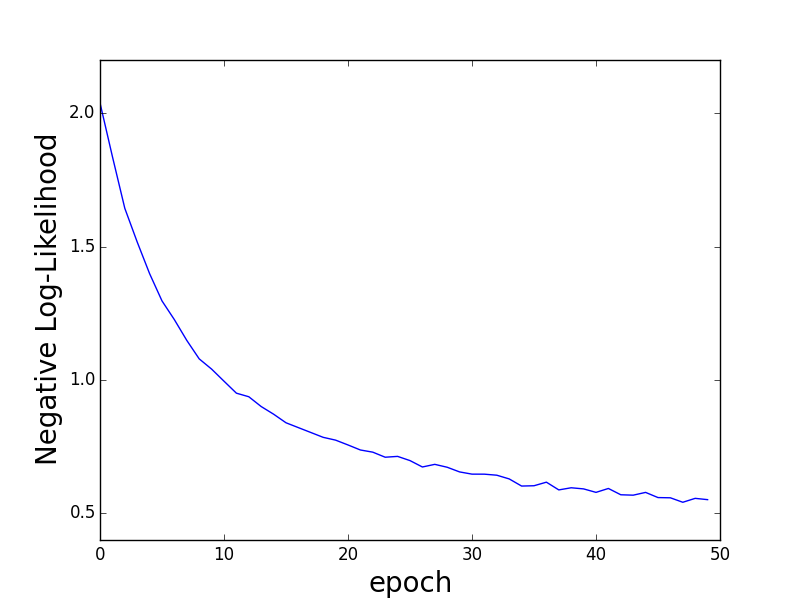
\includegraphics[width=\linewidth]{fig_mnist_nll.png}
  \caption{The negative log-likelihood}
  \label{fig:mnist_nll}
\end{subfigure}%
\begin{subfigure}{.45\textwidth}
  \centering
  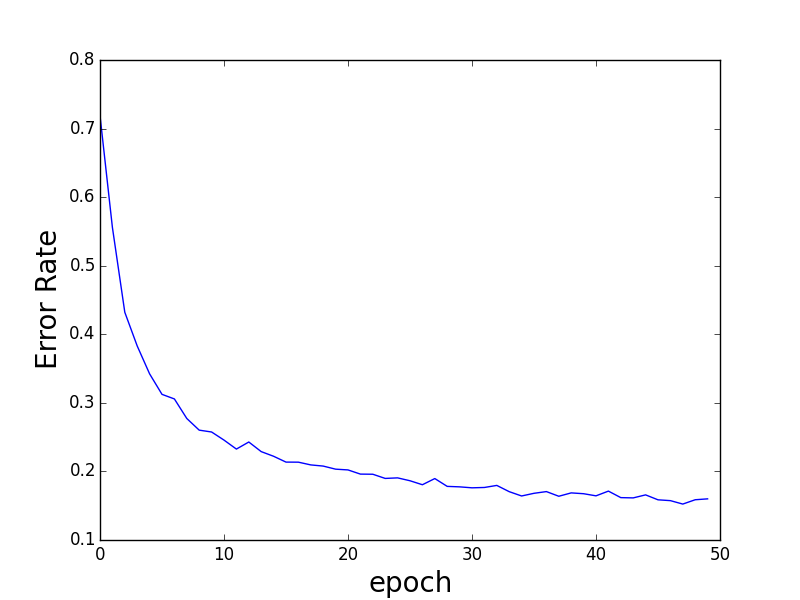
\includegraphics[width=\linewidth]{fig_mnist_err.png}
  \caption{The classification error rate}
  \label{fig:mnist_err}
\end{subfigure}
\caption{MNIST hand-written digits modeled using a two hidden
  layer neural network, with negative log-likelihood and
  classification error rate computed after each epoch.}
\label{fig:mnist_results}
\end{figure}
%
By increasing the number of epochs and a few minor modifications,
this model could potentially reach error rates as low as $2\%$.
However, this will not be explored since it is not
the main purpose of this document,
and optimization can be very time consuming due to computation.

% It is important to note that the activation function chosen is ReLU, 
% which is not easy to incorporate due within a 
% restricted Boltzmann machine context due to an unbounded range.
% However, a recently introduced method called 
% general adversarial networks can be used instead using the ReLU functions
% in alternative to restricted Boltzmann machines.
% This will be explored further in future discussions.

While the technique is more than a sufficient solution 
for recognizing hand-written digits,
naively applying gradient descent to more complex 
neural networks tend to have poor results.
Alternative methods will be discussed in the next section 
in order to address this problem.

Also note this type of neural networks is feed-forward, 
which mean it is limited to only supervised type problems
where the data structure is consistent 
and a prediction target (label) is provided for each sample.
For a collaborative filtering type problem,
the inference is often made within the data structure itself, 
which makes an unsupervised learning problem.
Feed-forward neural networks also fail to fully utilize 
the datasets that are partly labeled, 
known as semi-supervised problems.
These problems would require other variations of neural networks
with different methods for inference.





